\begin{figure}[!t]
    \centering
    % Define specific dimensions to ensure uniformity
    \newcommand{\figwidth}{0.49\columnwidth}
    \newcommand{\figheight}{5cm} % Adjust this value until the aspect ratio looks natural
    
    \begin{subfigure}[b]{\figwidth}
        \centering
        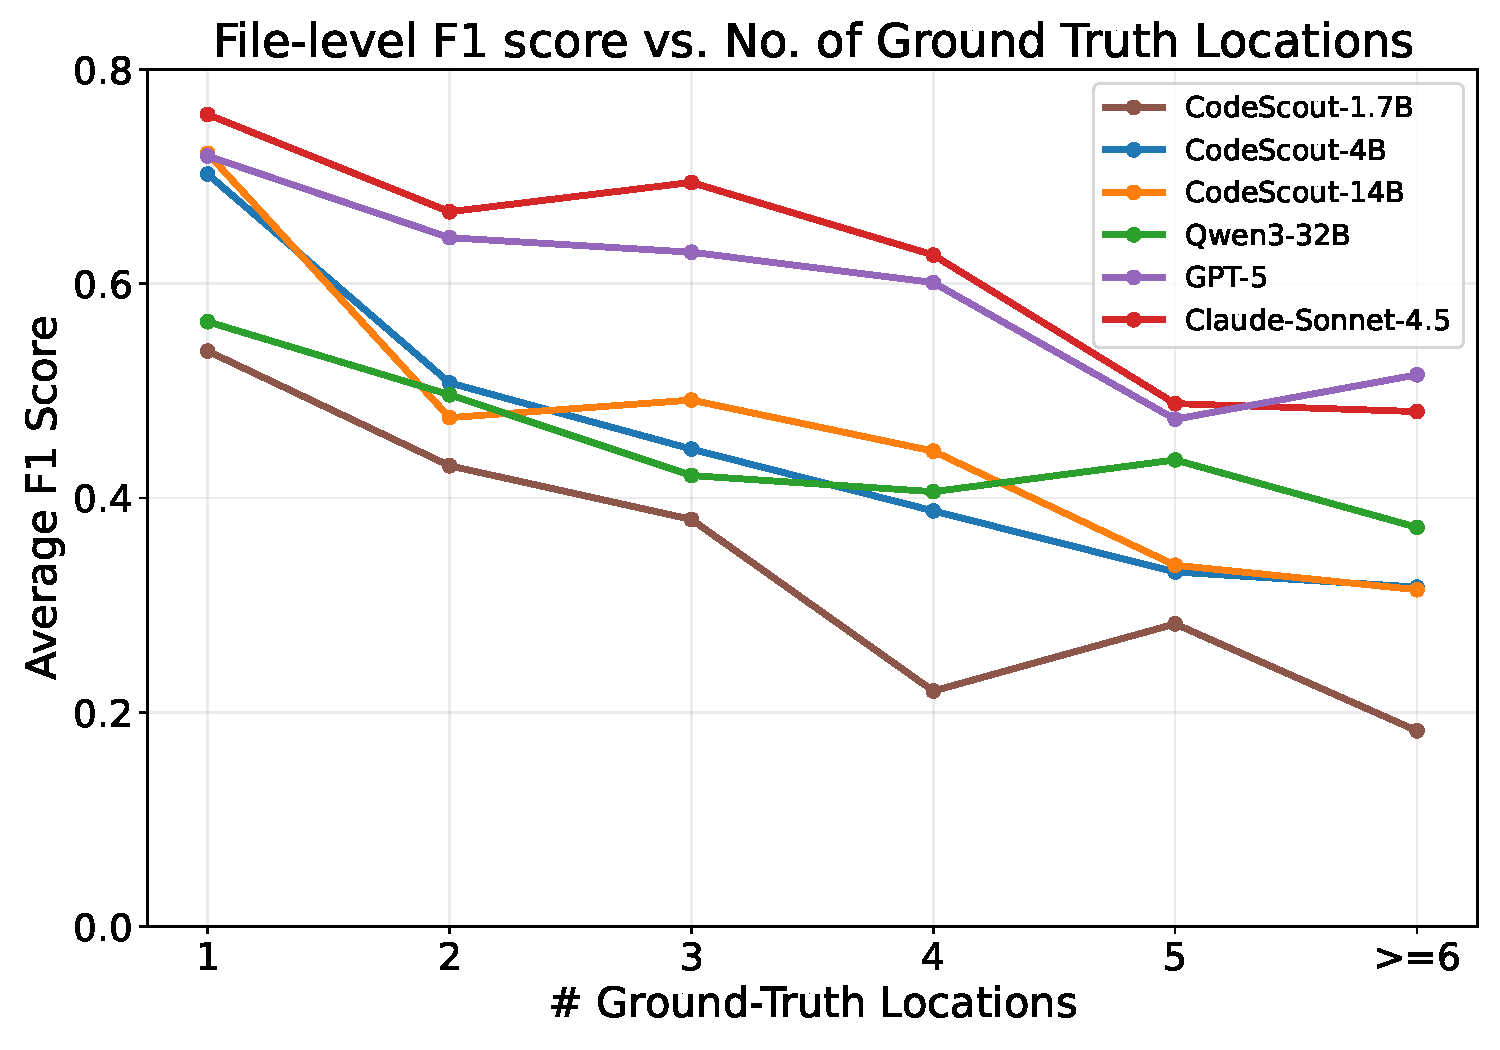
\includegraphics[width=\columnwidth, height=\figheight]{COLM/Figures/performance_vs_location_cnt_pro_file.pdf}
        % \caption{File-level F1 score vs. No. of Ground Truth Files on SWE-Bench Pro.}
        \label{fig:file_level_sub}
    \end{subfigure}
    \hfill
    \begin{subfigure}[b]{\figwidth}
        \centering
        % Specifying both height and width forces the images to match exactly
        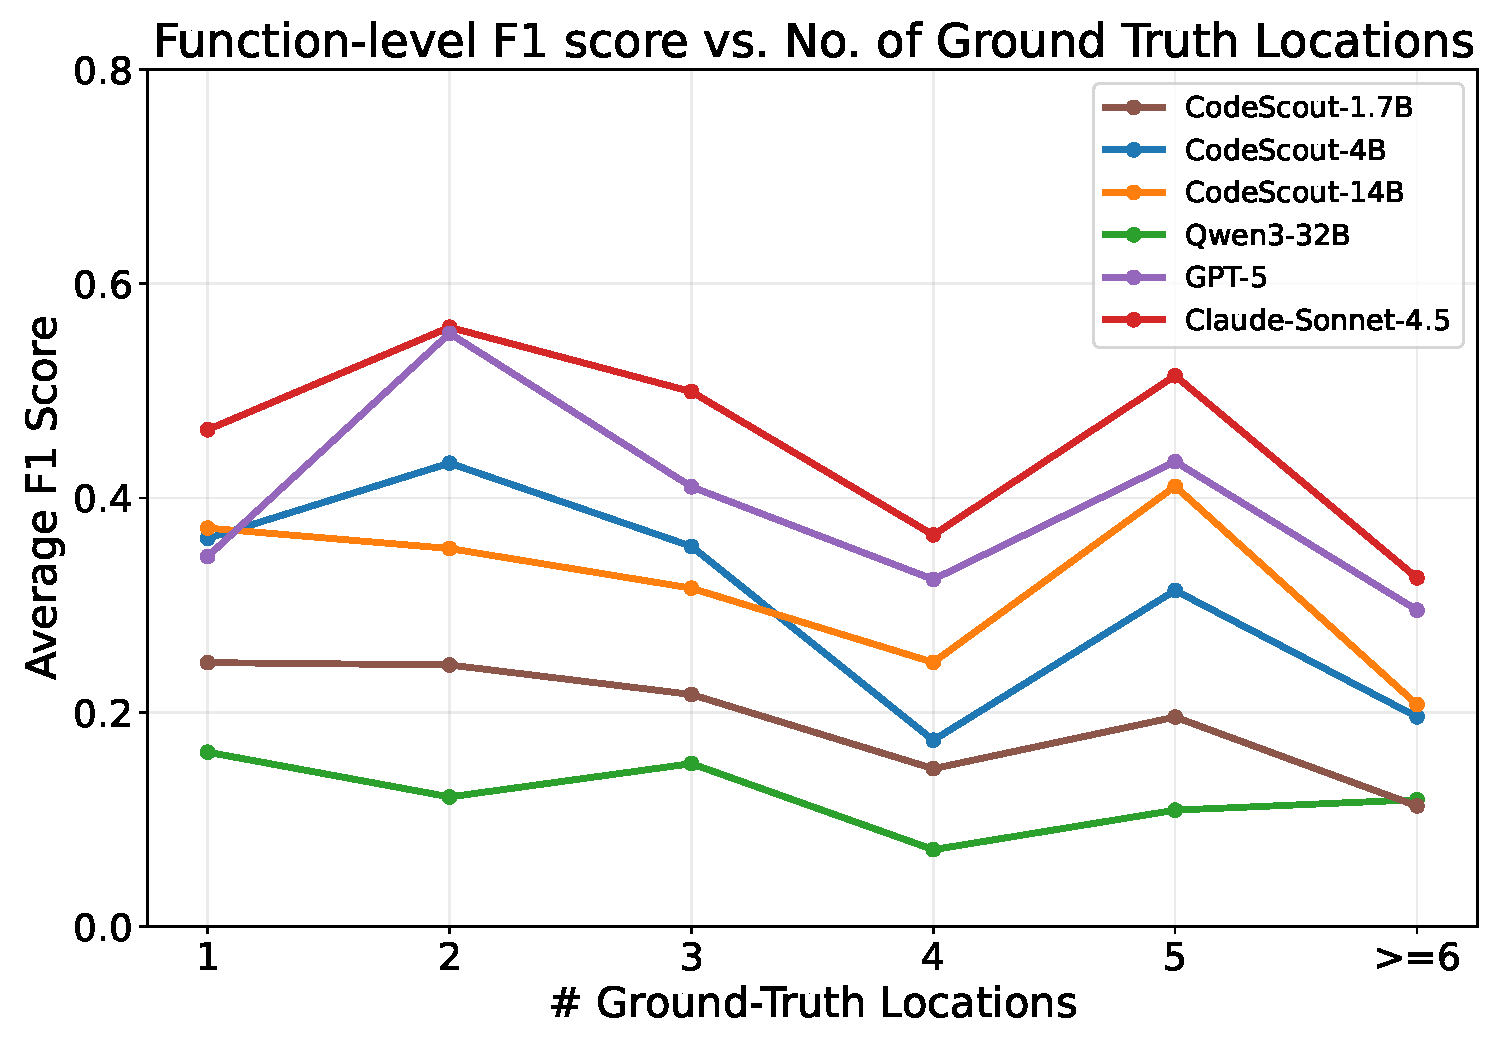
\includegraphics[width=\columnwidth, height=\figheight]{COLM/Figures/performance_vs_location_cnt_pro_function.pdf}
        % \caption{Function-level F1 score vs. No. of Ground Truth Functions on SWE-Bench Pro}
        \label{fig:function_level_sub}
    \end{subfigure}

    \caption{Average F1 score versus the number of locations edited by the ground truth issue resolution patch at the file-level (left) and function-level (right) on the SWE-Bench Pro dataset. The performance of all models drops as issues grow more complex with more files/functions being edited by the issue resolution patch.}
    \label{fig:performance_vs_locationcnt}
\end{figure}